% %%%% Benifit of reasoning about 
% \subsection{Motivation of Reasoning about Adaptivity}
% % 
\paragraph*{Introduction to Adaptivity Analysis}
Consider a dataset $X$ consisting of $n$ independent samples from some unknown population $\dist$.  How can I ensure that the conclusions drawn from $X$ \emph{generalize} to the population $\dist$?  Despite decades of research in statistics and machine learning on methods for ensuring generalization, there is an increased recognition that many scientific findings generalize poorly (e.g. 
\cite{Ioannidis05,GelmanL13}
).  While there are many reasons a conclusion might fail to generalize, one that is receiving increasing attention is \emph{adaptivity}, which occurs when the choice of method for analyzing the dataset depends on previous interactions with the same dataset~\cite{GelmanL13}.

 Adaptivity can arise from many common practices, such as exploratory data analysis, using the same data set for feature selection and regression, and the re-use of datasets across research projects.  Unfortunately, adaptivity invalidates traditional methods for ensuring generalization and statistical validity, which assume that the method is selected independently of the data. The misinterpretation of adaptively selected results has even been blamed for a ``statistical crisis'' in empirical science~\cite{GelmanL13}.
%  ~\cite{GelmanL13}.

A line of work initiated by \cite{DworkFHPRR15}, \cite{HardtU14} posed the question: Can I design \emph{general-purpose} methods that ensure generalization in the presence of adaptivity, together with guarantees on their accuracy?  
The idea that has emerged in these works is to use randomization to help ensure generalization. 
Specifically, these works have proposed to mediate the access of an adaptive data analysis to the data by means of queries from some pre-determined family (I will consider here a specific family of queries often called "statistical" or "linear" queries) that are sent to a 
\emph{mechanism} which uses some randomized process to guarantee that the result of the query does not depend too much on the specific
sampled dataset. 
%
\begin{figure}
    \centering
    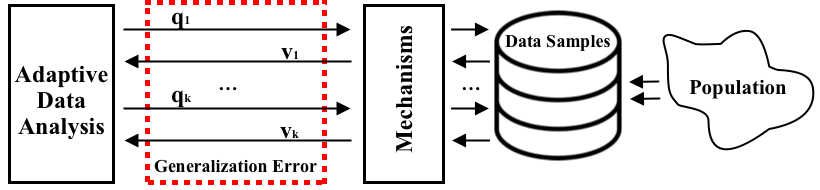
\includegraphics[width=0.7\columnwidth]{figures/data_analysis_model.png}
    \caption{Overview of our Adaptive Data Analysis model.}
    \label{fig:adaptivity-model-overview}
\vspace{-0.5cm}
\end{figure}
This guarantees that the result of the queries generalizes well. 
This approach is described in Figure~\ref{fig:adaptivity-model-overview}, where
I have a population that I'm interested in studying, and a dataset containing individual samples from this population. The adaptive data analysis I'm interested in running has access to the dataset through queries of some pre-determined family (e.g., statistical or linear queries) mediated by a mechanism. 
This mechanism uses randomization to reduce the generalization error of the queries issued to the data.
This line of work has identified many new algorithmic techniques for ensuring generalization in adaptive data analysis, leading to algorithms with greater statistical power than all previous approaches. 
Common methods proposed by these works include, the addition of noise to the result of a query, data splitting, etc. 
Moreover, these works have also identified problematic strategies for adaptive analysis, showing limitations on the statistical power one can hope to achieve. 
Subsequent works have then further extended the methods and techniques in this approach and further extended the theoretical underpinning of this approach, 
e.g.~\cite{dwork2015reusable,dwork2015generalization,BassilyNSSSU16,UllmanSNSS18,FeldmanS17,jung2019new,SteinkeZ20,RogersRSSTW20}.
%

A key development in this line of work is that the best method for ensuring generalization in an adaptive data analysis depends to a large extent on the number of \emph{rounds of adaptivity}, the depth of the chain of queries. 
As an informal example, the program $x \leftarrow \query_1(D);y \leftarrow \query_2(D,x);z \leftarrow \query_3(D,y)$ has three rounds of adaptivity, since $\query_2$  depends on $D$ not only directly because it is one of its input but also via the result of $\query_1$, 
which is also run on $D$, and similarly,  $\query_3$ depends on $D$ directly but also via the result of $\query_2$, which in turn depends on the result of $\query_1$. 
The works I discussed above showed that, not only does the analysis of the generalization error depend on the number of rounds, 
but knowing the number of rounds actually allows one to choose methods that lead to the smallest possible generalization error. 

% \mg{Check the following - also the plots need to be on the same scale!}
For example, these works showed that when an adaptive data analysis use a large number of rounds of adaptivity then a low generalization error can be achieved by mechanism of 
adding to the result of each query Gaussian noise scaled to the number of rounds. When instead  an adaptive data analysis uses a small number of rounds of adaptivity then a low generalization error can be achieved by using more specialized methods, such as data splitting mechanism or the reusable holdout technique from~\cite{DworkFHPRR15}.
To better understand this idea, I show in Figure~\ref{fig:generalization_errors} two experiments showcasing these situations. 
More precisely, in Figure~\ref{fig:generalization_errors}(a) shows the results of a real world analysis
with two rounds of adaptivity. 
This analysis can be seen as a classifier which first runs 500 non-adaptive queries on the first 500 attributes of the data, looking for correlations between the attributes and a label, and then runs one last query which depends on all these correlations. 
Without any mechanism the generalization error is pretty large, and the lower generalization error is achieved when the data-splitting method is used. 
In Figure~\ref{fig:generalization_errors}(b) shows the results of a specific analysis
with four hundreds rounds of adaptivity. 
This analysis can be seen as a classifier which at each step runs an adaptive query based on the result of the previous ones. 
Again, without any mechanism the generalization error is pretty large, and the lower generalization error is achieved when the Gaussian noise is used. 
{\small
\begin{figure}
\centering
\begin{subfigure}{.48\textwidth}
\begin{centering}
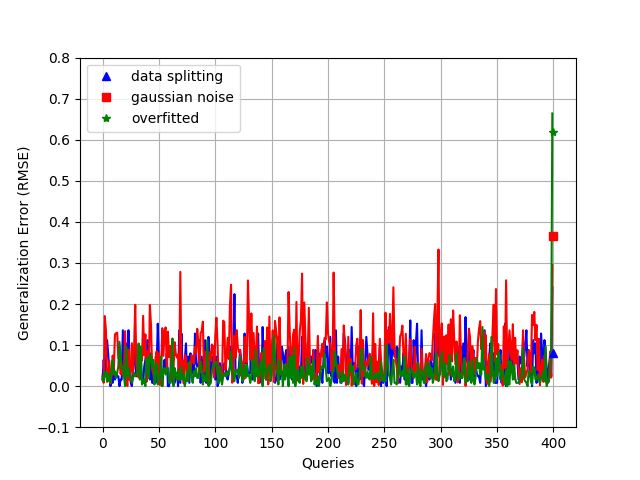
\includegraphics[width=0.9\textwidth]{figures/tworound.png}
\caption{}
\end{centering}
\end{subfigure}
%}
\quad
\begin{subfigure}{.48\textwidth}
\begin{centering}
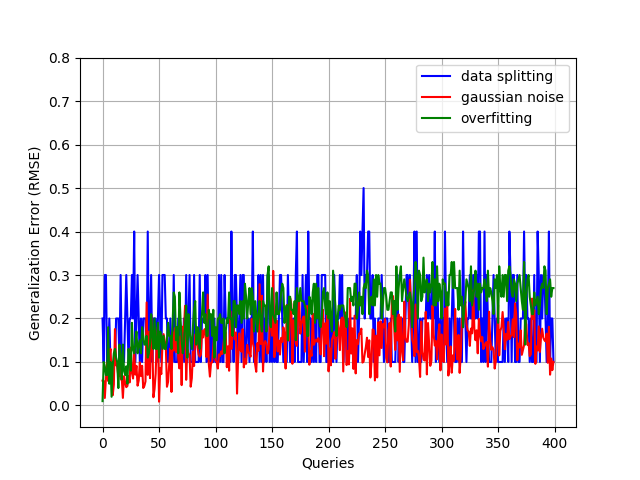
\includegraphics[width=0.9\textwidth]{figures/multipleround.png}
\caption{}
\end{centering}
\end{subfigure}
\vspace{-0.4cm}
 \caption{
 The generalization errors of two adaptive data analysis examples, under different choices of mechanisms.
 (a) Data analysis with adaptivity 2, 
 (b) Data analysis with adaptivity 400. 
}
\label{fig:generalization_errors}
\vspace{-0.5cm}
\end{figure}
}
%gap
This scenario motivates us to explore the design of program analysis techniques that can be used to estimate the number of \emph{rounds of adaptivity} that a program implementing a data analysis can perform. These techniques could be used to help a data analyst in the choice of the mechanism to use,
and they
could be ultimately be integrated into a tool for adaptive data analysis such as the \emph{Guess and Check} framework by~\cite{RogersRSSTW20}. 
%
In order to analyze this property, there are mainly three property. 
In this proposal, I will first focus on analyzing 
this adaptivity property for program based on solving the three problems specifically as follows.

\paragraph*{Adaptivity Analysis}
There are mainly three problems in order to analyse this adaptivity property, 
and the full-spectrum analysis on this property is 
% In this proposal, I will first focus on analyzing 
% this adaptivity property for program based on solving 
developed w.r.t. the three problems specifically as follows.

\begin{itemize}
    \item
The first problem is \emph{how to define formally} a model for adaptive data analysis which is general enough to support the methods I discussed above and would permit to formulate the notion of adaptivity these methods use. 
I take the approach of designing a programming framework for submitting queries to some \emph{mechanism} giving access to the data mediated by one of the techniques I mentioned before, e.g., adding Gaussian noise, randomly selecting a subset of the data, using the reusable holdout technique, etc. 
In this approach, a program models an \emph{analyst} asking a sequence of queries to the mechanism. The mechanism runs the queries on the data applying one of the methods discussed above and returns the result to the program. The program can then use this result to decide which query to run next. 
% Overall, I'm interested in controlling the generalization of the results of the queries which are returned by the mechanism, by means of the adaptivity. 

Motivated by this, I present a while-like language with extensions on query request in Section~\ref{sec:language}.

\item 
The second problem is \emph{how to define the adaptivity of a given program}.
Intuitively, a query $Q$ may depend on another query $P$, if there are two values that $P$ can return which affect in different ways the execution of $Q$. 
For example, as shown in \cite{dwork2015reusable}, and as I did in our example in Figure~\ref{fig:generalization_errors}(a), one can design a machine learning algorithm for constructing a classifier which first computes each feature's correlations with the label via a sequence of queries, and then constructs the classifier based on the correlation values. 
If one feature's correlation changes, the classifier depending on features is also affected.  
This notion of dependency builds on the execution trace as a \emph{causal history}. 
In particular, I'm interested in the history or provenance of a query up until this is executed, I'm not then concerned about how the result is used --- except for tracking whether the result of the query may further cause some other query. 
This is because I focus on the generalization error of queries and not their post-processing. % 
To formalize this intuition as a quantitative program property, I develop an execution-based analysis
% I first consider all the possible evaluations of a programs  --- I do this by 
% I use a trace semantics recording the execution history of programs on some given input --- and I create a dependency graph, where the dependency between different variables (query is also assigned to variable) is explicit and track which variable is associated with a query request. 
% I then enrich this graph with weights describing the maximal number of times each variable is evaluated in a program evaluation starting with an initial state. The adaptivity is then defined as the length of the walk visiting most query-related variables on this graph. 
% Through two aspects: the execution-based analysis and static-based program analysis.
% 	In the execution-based analysis, I will formalize the intuitive notion of \emph{adaptivity} as a quantitative 
%    property of programs. This analysis is developed 
   in three steps through different methodologies in each step as follows,
   \begin{enumerate}
	\item The dependency relation between every query, through the methodology of semantic data dependency analysis.
    \\
    Specifically through a trace semantics recording the execution history of programs on some given input
    %  --- and I create a dependency graph, 
     the dependency between different variables (query is also assigned to variable) is explicit and track which variable is associated with a query request. 
% I then enrich this graph with weights describing the maximal number of times each variable is evaluated in a program evaluation starting with an initial state. The adaptivity is then defined as the length of the walk visiting most query-related variables on this graph. 
% 	In the execution-based analysis, I will formalize the intuitive notion of \emph{adaptivity} as a quantitative 
%    property of programs. This analysis is developed 
%    \\
   \item The dependency quantity analysis, through the methodology of execution-based data reachability bound analysis.
%    \\
	\item The adaptivity quantity analysis, based on the two analysis results above, give the formal \emph{adaptivity} model 
   for program.
   \\
   Specifically, I create a dependency graph, where the dependency between different variables (query is also assigned to variable) is explicit and track which variable is associated with a query request. 
   I then enrich this graph with weights describing the maximal number of times each variable is evaluated in a program evaluation starting with an initial state. 
   The adaptivity is then defined as the length of the walk visiting most query-related variables on this graph. 
   \end{enumerate}
\item 
The third problem is \emph{how to estimate the adaptivity of a given program}. 
The adaptive data analysis model I consider and our definition of adaptivity suggest that for this task I can use a  program analysis that is based on some form of dependency analysis. This analysis needs to take into consideration:
1) the fact that, in general, a query $Q$ is not a monolithic block but rather it may depend, through the use of variables and values, on other parts of the program. 
Hence, it needs to consider some form of data flow analysis. 
2) the fact that, in general, the decision on whether to run a query or not may depend on some other value. Hence, 
 it needs to consider some form of control flow analysis.
3) the fact that. in general, I'm not only interested in whether there is a dependency or not, but in the length of the chain of dependencies. 
Hence, it needs to consider some quantitative information about the program dependencies. % {A quick example is that : I store the result of query $Q_1$ in variable $x$ and use variable $y$ to record the result of query $Q_2$. I want to construct the third query $Q_3$ which relies on the value stored in $x$, let us say, $Q_3$ will ask for the sum of the first column of a table if $x$ is positive and the sum of the second column otherwise. In this situation, I need data flow analysis. On the other hand, if I need the value of $y$ to help us decide whether I should ask $Q_3$, for example, I ask the third query if $y$ is odd, and do not ask if $y$ is even. Naturally, to be able to handle this case, control flow analysis comes into play. Formally speaking,  }
To address these considerations and be able to estimate a sound upper bound on the adaptivity of a program, 
I will develop a program analysis algorithm, named {\THESYSTEM}, which combines data flow and control flow analysis with reachability bound analysis~\cite{GulwaniZ10}. 
This new program analysis gives tighter bounds on the adaptivity of a program than the ones one would achieve by directly using the data and control flow analyses or the ones that one would achieve by directly using reachability bound analysis techniques alone. Specifically as follows in the same 3 aspects as the execution-based analysis 
while through static program analysis techniques, and a sound estimated result will be given in each aspect as follows.
\begin{enumerate}
\item The data dependency relation analysis through the static data flow analysis technique.
\item The dependency quantity analysis through the static program reachability bound analysis techniques.
\item The program adaptivity estimation, through newly designed algorithms based on the results estimated above, 
computing the adaptivity upper bound soundly 
and accurately.
\end{enumerate}
%%%%% To reason about
\end{itemize}
I will implement my program analysis and show that it can help to analyze the adaptivity of several concrete data analyses with different adaptivity structures.
% \\
\paragraph*{Towards the Accurate Program Resource Cost Analysis}
Then, motivated by the two following aspects,  I'm interested in improving the accuracy of program's general resource cost analysis
by generalizing my \emph{adaptivity} analysis framework.
\begin{itemize}
    \item Firstly, in traditional program's resource cost analysis,
    There are two categories of the program cost analysis, type-system based  and data-flow/control-flow analysis based. 
    In the type-system design based works, they \cite{GustafssonEL05} and \cite{hoffmann_jost_2022}, explicit abstraction or data structure de-allocation in order to save or reduce the cost.
    
    Both of the
    works in these two areas fails to recognize the case where program resource consumption is decreased implicitly.
    \item The resource consumption during the program 
    execution increases and particularly decreases implicitly in the same way as the program's adaptivity. This is explained in detail through an example in Section~\ref*{sec:generalization}.
\end{itemize}
% F
% Then, through two observations,
%    that 
%    firstly, traditional program's resource cost analysis they failed to consider the case where the program's cost could decrease 
%    implicitly, and 
%    % when there isn't a dependency relation between variables.
%    the resource consumption during the program 
%    execution increases and particularly decreases implicitly in the same way as the program's adaptivity, 
%    % Specifically, in line 5 
%    % where the list is re-written and the heap consumption is decreased implicitly. 
%    % This implicit decrease 
%    % of the cost works exactly the same as program's adaptivity decrease.
%    I'm interested in improving the accuracy of program's general resource cost analysis
%    by generalizing my \emph{adaptivity} analysis framework.
   %  onto the program's resource cost analysis. 
   % Use this framework,
   Based on the observations above, and through the generalized \emph{adaptivity} analysis framework.
   I will give
   a more accurate resource cost estimation by taking the program's implicit resource cost into consideration, comparing 
   to the worst case cost analysis in traditional way.

   \paragraph*{Towards Solving the CFL-Reachability Problem}
Finally, based on the study on traditional way of performing data flow and control analysis,
I identify the similarity between the traditional way of performing data flow and control analysis, and the 
   adaptivity analysis.  
   Specifically I identify the similarity between 
   solving the feasible path problem in the analysis by reducing to CFL-reachability problems,
   and the way of computing the adaptivity in my static analysis framework.
   Motivated by this observation, 
   % I'm insterested
   % the, There are similarity between
   % solving the data flow problem by reducing to CFL-reachability problem,
   % resource analysis through reducing to CFL-reachability problem, 
   I'm interested in showing that
   CFL-reachability problems can be solved by reducing it into my adaptivity analysis framework.

   \section{Contributions}

   Program analysis techniques are usually applied to study quantitative properties. In comparison to those related works, this dissertation has the following contributions.
   
   \begin{enumerate}
   
   \item We propose a formal definition of the adaptivity of adaptive data analysis programs and develop a graph-based program analysis algorithm that statically estimates the adaptivity.
   \item reachability bound computing algorithm
   % To the best of our knowledge, it is the first work that statically estimates adaptivity to help design adaptive data analysis algorithms.  
   \end{enumerate}

%%%%% To reason about
\section{Methodology}
We use static analysis techniques to reason about the two main quantitative properties studied in this dissertation: 
the adaptivity of adaptive data analysis programs,
the reachability bound of while loop programs. 

\subsection{Abstract Interpretation}

\subsection{Dependency Graph}
Another quantitative property we study is the adaptivity of adaptive data analysis programs. 
{The adaptivity is defined to be the length of the longest chain of queries of the program in which one query may rely 
on its previous queries in the same chain. 
The adaptivity of a data analysis program is quite different from the relative cost of the two programs. To reason about cost, we can simply sum the costs of sub-programs to get the upper bound of the cost. However, the adaptivity of each sub-program of the target program does not help much in finding the adaptivity. To use a type and effect system to reason about adaptivity, this system should be able to express certain dependencies.
% Of course, we can sum them but then the result becomes imprecise. For this reason, we think the type and effect system is not the good direction to reason about the adaptivity of a data analysis program since it is tricky for the effect to carry information such as one query may depend on the other one. 
We expect adaptivity can also be reasoned about by type and effect systems but in this work, we choose to use a dependency graph to reason about adaptivity.}

{There are two challenges to reason about adaptivity: what will a formal definition of the adaptivity of a data analysis program look like, and how to reason about the adaptivity. 
In our work, the first challenge is solved by a query-based dependency graph generated along with the evaluation of the program. 
Our trace-based operational semantics can generate the trace which tracks the queries asked in the evaluation of the program. 
The query-based dependency graph is constructed based on the queries in the trace. Every node of the graph represents a unique query asked in the program, and the directed edge between two nodes, identifying one query (one node) may depend on the other one. 
The adaptivity is then formally defined as the length of the longest path in the query-based dependency graph.}
{The second challenge is how to estimate the adaptivity of a data analysis program we have just defined. 
In order to upper bound the length of the longest path in the query-based dependency graph, we want to find a path in a dependency graph as well such that the path contains all the queries in that longest path in the query-based dependency graph. 
We develop an algorithm to build a variable-based dependency graph, in which every node represents the unique variable that is assigned in one assignment statement of the program. 
The direct edge between two nodes reflects both the data dependency and control flow dependency between variables. Also, we add the unit weight to the node whose variable is associated with a query result. Then the upper bound on the adaptivity of the data analysis program is estimated by the weight of the path with the highest weights in the variable-based dependency graph.}

{To summarize, we use two dependency graphs for reasoning about the adaptivity of a data analysis program: 
one query-based dependency graph to define the adaptivity, and one weighted variable-based dependency graph to estimate an upper bound on the adaptivity. }



\section{Dissertation Outline}
This dissertation includes two main parts. 
\begin{enumerate}
\item A while-like language extended with query request feature, named {\tt Query While} Language, 
used to implement 
the adaptive data analysis.
\item A formal adaptivity model through execution-based adaptivity analysis.
\item A static program analysis algorithm, named {\THESYSTEM}.
\item Two proposed further features to be improved based-on the formal adaptivity model and {\THESYSTEM},
 expected to be done before the final defense.
\item A proposed accurate program resource cost analysis framework generalized from {\THESYSTEM}. 
The analysis framework design is expected to be done with the implementation start off before final defense.
\item A proposed plan for solving the CFL-reachability problem via reduction into the {\THESYSTEM} framework,
expected to be started off before final defense and developing further sophisticated after.
\end{enumerate}



\section{Previous Published Material}
The contents of this dissertation are partly based on the work and writing in the following papers.

% The work of{\ADAPTSYSTEM} is still under preparation.


